 In this model, we suppose that the data was generated using linear recursive formula
 \begin{equation}
  \label{eq:varx_stationary}
	x_t = \mu + \sum\limits_{q=1}^{\mathrm{xmem}} A_q x_{t-q} + \sum\limits_{p=0}^{\mathrm{umem}} B_p u_{t-p} + \varepsilon_t, \forall t = \mathrm{xmem}, \mathrm{xmem}+1, \dots, T-1,
 \end{equation}
 where given data $x_t \in \mathbb{R}^{\mathrm{xdim}}, t = 0,\dots,T-1$ are stored in column vectors, $A_q \in \mathbb{R}^{\mathrm{xdim},\mathrm{xdim}}$ are unknown coefficients (matrices) corresponding to previous $\mathrm{xmem}$ time-steps and \todo{write here something funny about variables in the model}.
  
 Let us denote the number of equations in \eqref{eq:varx_stationary} by $m = T-\mathrm{xmem}$.
 Moreover, we define 
 \begin{displaymath}
  \begin{array}{rcl}
   X & = & [x_{\mathrm{xmem}}, x_{\mathrm{xmem}+1}, \dots, x_{T-1}] \in \mathbb{R}^{\mathrm{xdim},m} \\[5mm]
   M & = & [\mu, A_1, A_2, \dots, A_{\mathrm{xmem}}, B_0, B_1, \dots, B_{\mathrm{umem}} ] \in \mathbb{R}^{\mathrm{xdim},1+\mathrm{xmem}\cdot\mathrm{xdim}+(\mathrm{umem}+1)\cdot\mathrm{udim}}\\[5mm]
   Z & = & \left[
	\begin{array}{ccccc}
	 1 & 1 & 1 & & 1 \\ \hdashline[2pt/2pt]
	 x_{\mathrm{xmem}-1} & x_{\mathrm{xmem}} & x_{\mathrm{xmem}+1} & & x_{T-1} \\
	 \vdots & \vdots & \vdots & \dots & \vdots \\
	 x_0 & x_1 & x_2 & & x_{T-\mathrm{xmem}} \\ \hdashline[2pt/2pt]
	 u_{\mathrm{xmem}} & u_{\mathrm{xmem}+1} & u_{\mathrm{xmem}+2} & & u_{T-1} \\
	 u_{\mathrm{xmem}-1} & u_{\mathrm{xmem}} & u_{\mathrm{xmem}+1} & & u_{T-2} \\
	 \vdots & \vdots & \vdots & & \vdots 
    \end{array}
   \right] \in \mathbb{R}^{1+\mathrm{xmem}\cdot\mathrm{xdim}+(\mathrm{umem}+1)\cdot\mathrm{udim},m} \\[5mm]
   \varepsilon & = & [\varepsilon_{\mathrm{xmem}}, \varepsilon_{\mathrm{xmem}+1}, \dots, \varepsilon_{T-1}] \in \mathbb{R}^{\mathrm{xdim},m}
  \end{array}
 \end{displaymath}

 Then \eqref{eq:varx_stationary} is equivalent to\footnote{please, notice that both of left side and right side are matrices}
 \begin{equation}
  \label{eq:varx_stationary_matrix}
  X = MZ + \varepsilon,
 \end{equation}
 where $M$ is matrix of unknown parameters of the model \eqref{eq:varx_stationary}.
 Now we will find $M$ as \emph{the best} solution, i.e. we minimize the size of error $\varepsilon$ in \eqref{eq:varx_stationary_matrix}\footnote{please, notice that we are talking about matrix norms}
 \begin{displaymath}
  \label{eq:eq:varx_stationary_matrix_eps}
  \Vert \varepsilon \Vert = \Vert X - MZ \Vert ~~ \rightarrow ~~ \min\limits_{M}.
 \end{displaymath}
 or equivalently\footnote{\todo{the trace and matrix norms should be discussed}}
 \begin{displaymath}
   \bar{M} =  \arg \min\limits_{M} \Vert X - MZ \Vert =  \arg \Vert X - MZ \Vert^2 =  \arg \min\limits_{M} \underbrace{\tr\Vert X - MZ \Vert^2}_{= L(M)}.
 \end{displaymath}
 The optimization problem with object function $L(M): \mathbb{R}^{\mathrm{xdim},1+\mathrm{xmem}\cdot\mathrm{xdim}+(\mathrm{umem}+1)\cdot\mathrm{udim}} \rightarrow \mathbb{R}^{+}_0$ could be simplified 
 \begin{displaymath}
  \begin{array}{rcl}
   \min L(M) & = & \min \tr \Vert X - MZ \Vert^2 = \min \tr (X-MZ)^T(X-MZ) \\
        & = & \min \tr \left( X^TX - X^TMZ - (MZ)^TX + (MZ)^T MZ \right) \\
        & = & \min \tr \left( X^TX - X^TMZ - Z^TM^TX + Z^T M^T MZ \right) \\
        & = & \min \tr (X^TX) - \tr (X^TMZ) - \tr (Z^TM^TX) + \tr (Z^T M^T MZ)
  \end{array}
 \end{displaymath}
 We consider the neccessary optimality condition $\frac{\partial L(M)}{\partial M} = 0$, therefore we have to compute the derivatives of addends in the previous formula.
 These derivatives follow (using \cite{matrix_cookbook}\todo{add cookbook reference}).
 \begin{displaymath}
  \begin{array}{rcl}
   \frac{\partial \tr (X^TX)}{\partial M} & = & 0 \\
   \frac{\partial \tr (X^TMZ)}{\partial M} & = & XZ^T \\
   \frac{\partial \tr (Z^TM^TX)}{\partial M} & = & XZ^T \\
   \frac{\partial \tr (Z^TM^T M Z)}{\partial M} & = & M(ZZ^T) + M (ZZ^T) = 2MZZ^T
  \end{array}
 \end{displaymath}
 Therefore the neccessary optimality condition of the problem \eqref{eq:eq:varx_stationary_matrix_eps} is given by
 \begin{displaymath}
  \frac{\partial L(M)}{\partial M} = 0 ~~~ \Leftrightarrow ~~~ -2XZ^T + 2M(ZZ^T) = 0,
 \end{displaymath}
 which could be written in the form of the system of linear equations with multiple right-hand side vectors as
 \begin{equation}
  \label{eq:varx_stationary_system}
  (ZZ^T) M^T = ZX^T,
 \end{equation}
 where $M^T$ is the matrix of unknown parameters of the original model \eqref{eq:varx_stationary}.

 \subsection{Checking equations by example}
 
 Let us consider a problem with $\mathrm{xdim} = 2, \mathrm{udim} = 1, \mathrm{xmem} = 2, \mathrm{umem} = 0, T = 5$. Then $m = 3$ and
 \begin{displaymath}
  X \in \mathbb{R}^{2,3}, ~ M \in \mathbb{R}^{2,6}, ~ Z \in \mathbb{R}^{6,3}, ~\varepsilon \in \mathbb{R}^{2,3}.
 \end{displaymath}
 Please, see Fig. \ref{fig:varx1}, where we present given data (time-series and external forces) and Fig. \ref{fig:varx2} to visualize objects in the problem.
 
 \begin{figure}[h!]
  \centering
    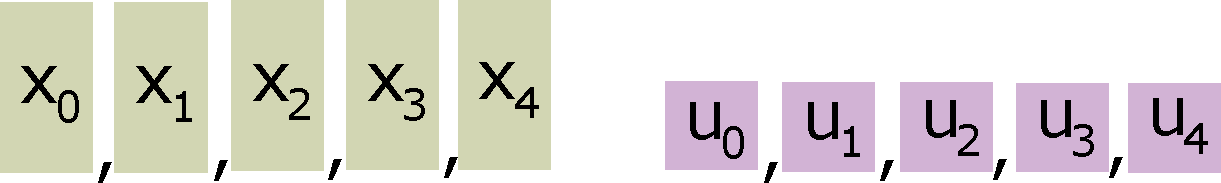
\includegraphics[scale=0.2]{figure/varx1.pdf}
  \caption{Given data in VarX problem; time-series values $x_0,x_1,x_2,x_3,x_4$ and external forces $u_0,u_1,u_2,u_3,u_4$.}
  \label{fig:varx1}
 \end{figure}

 \begin{figure}[h!]
  \centering
    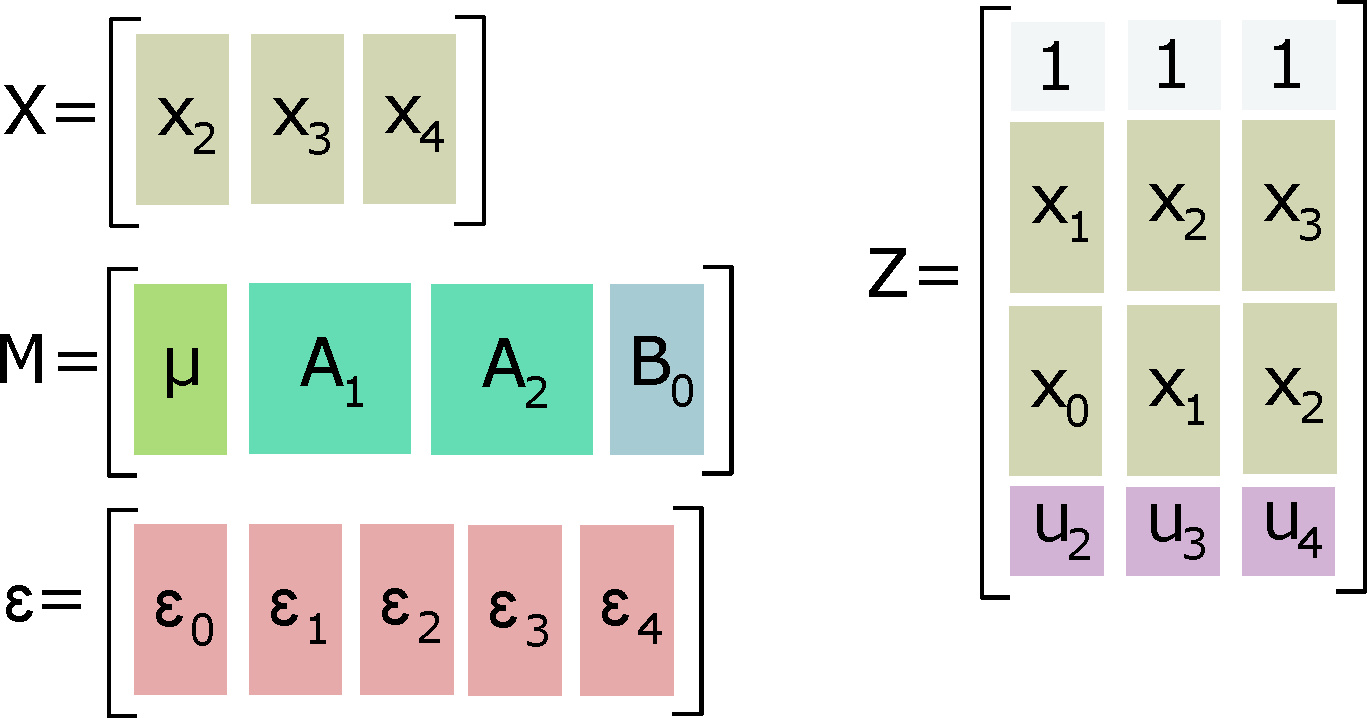
\includegraphics[scale=0.2]{figure/varx2.pdf}
  \caption{Objects in the VarX problem.}
  \label{fig:varx2}
 \end{figure}

 The most complicated operation in equation \eqref{eq:varx_stationary_matrix} is matrix multiplication $MZ$. The graphical analysis of this operation could be found in Fig. \ref{fig:varx3}.
 Here, we used general property
 \begin{displaymath}
  \forall A \in \mathbb{R}^{m,n} \forall v_1,v_2 \in \mathbb{R}^n: A\left[ v_1, v_2 \right ] = \left[ A v_1, Av_2 \right] ,
 \end{displaymath}
 i.e. multiplication by matrix could be applied into columns.

 \begin{figure}[h!]
  \centering
    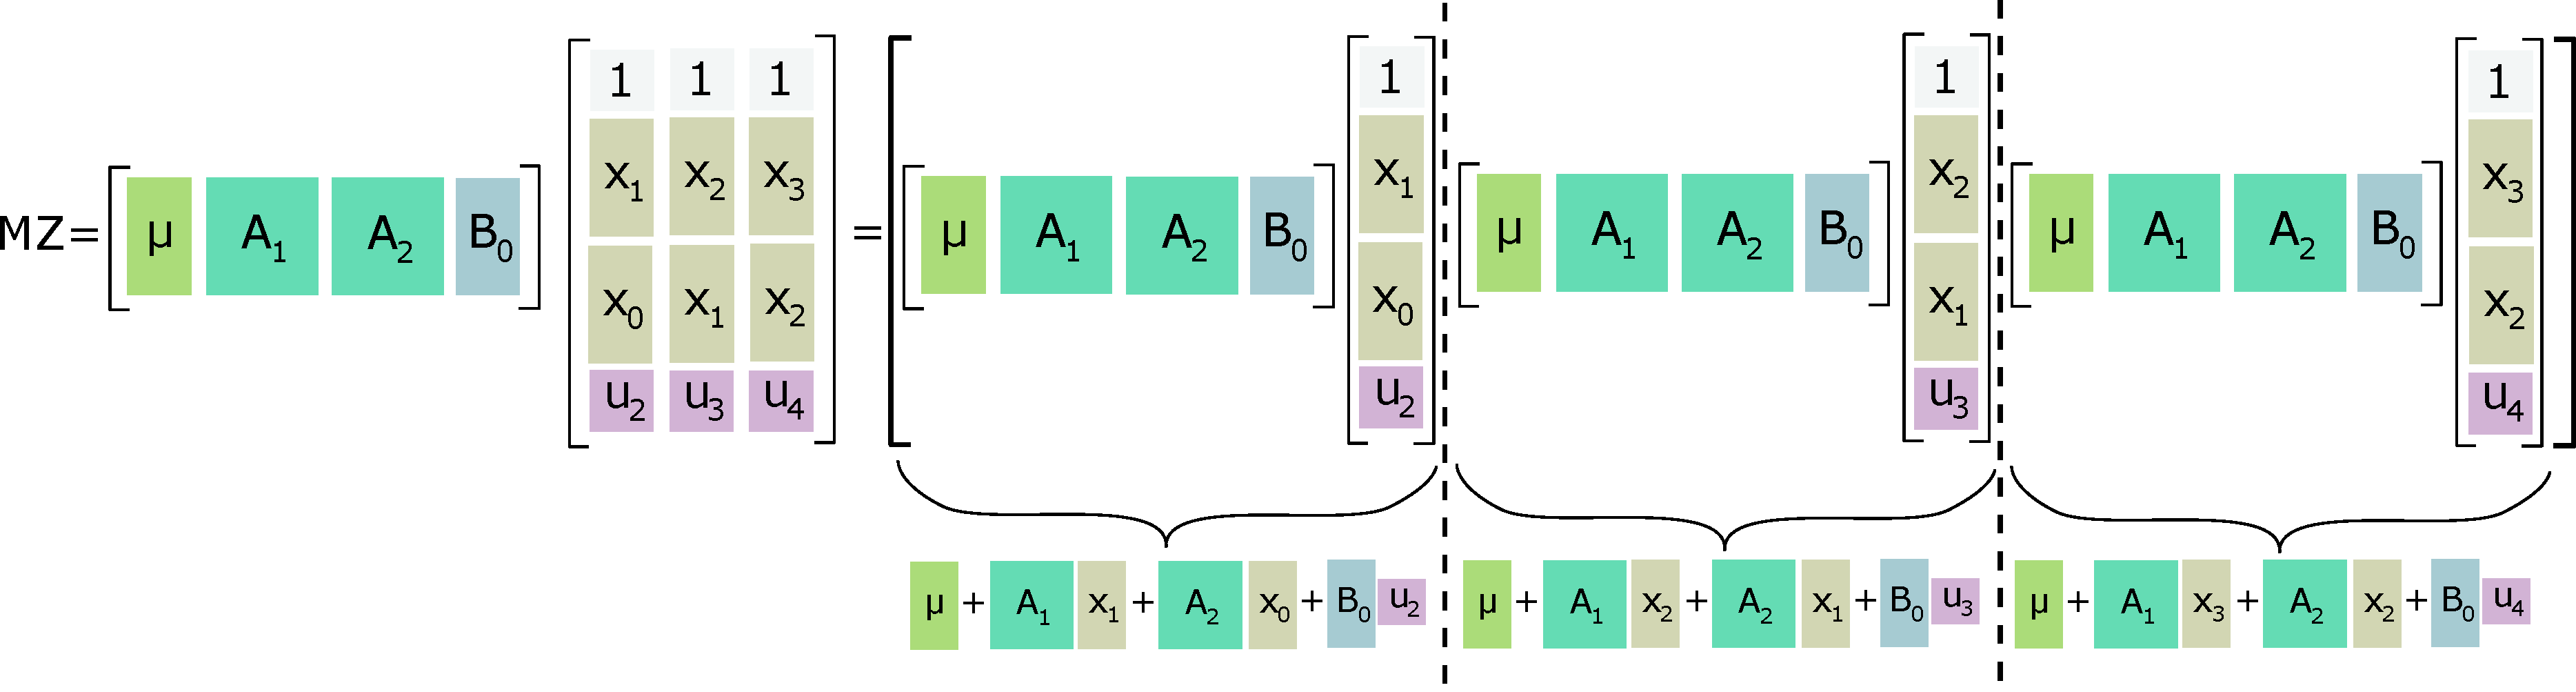
\includegraphics[scale=0.2]{figure/varx3.pdf}
  \caption{Multiplication $MZ$; the dashed line represents the separation between columns.}
  \label{fig:varx3}
 \end{figure}
 
 Now we are ready to assemble $X = MZ + \varepsilon$ (which we actually will not demonstrate, because the operation addition on the right side is an operation between columns of matrices, it is trivial, and it will be clear from following).
 Afterwards, we can compare columns on the left and right side of equation $X = MZ + \varepsilon$, see Fig. \ref{fig:varx4} and we obtain the original equations in VarX model, see equations \eqref{eq:varx_stationary}.
 Therefore, in this case, equations \eqref{eq:varx_stationary} and \eqref{eq:varx_stationary_matrix} are equivalent.

 \begin{figure}[h!]
  \centering
    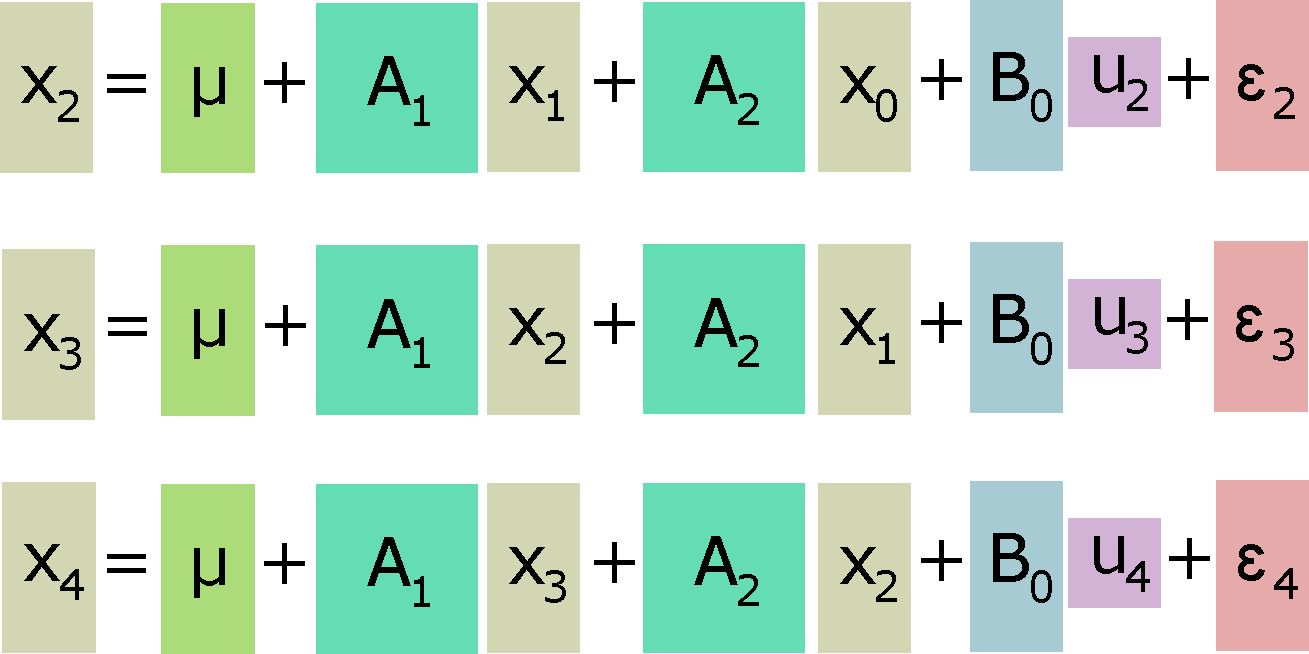
\includegraphics[scale=0.2]{figure/varx4.pdf}
  \caption{The definition of original VarX problem.}
  \label{fig:varx4}
 \end{figure}
